\documentclass[dvipsnames,beamer,10pt]{standalone}

\usepackage{textcomp}
\usepackage{lmodern}

\usepackage{textcomp}
\usepackage{lmodern}

\usepackage{tikz}
\usepackage{arrayjob}




\usetikzlibrary{positioning,decorations.pathreplacing,fit}
\usetikzlibrary{decorations.markings,arrows.meta,shapes.arrows,arrows}
\usetikzlibrary{bending}
\usetikzlibrary{calc}

\definecolor{mygreen}{RGB}{0,128,80}
\colorlet{darkgreen}{mygreen!90!black}

\providecommand{\adlog}{\textcolor{red}{a}}
\providecommand{\bdlog}{\textcolor{blue}{b}}
\providecommand{\cdlog}{\textcolor{Plum}{c}}
\providecommand{\ddlog}{\textcolor{OliveGreen}{d}}
\providecommand{\dlog}[2]{\textcolor{#1}{#2}}
\providecommand{\ua}[1]{\dlog{red}{#1}}
\providecommand{\ub}[1]{\dlog{blue}{#1}}
\providecommand{\uc}[1]{\dlog{Plum}{#1}}
\providecommand{\ud}[1]{\dlog{OliveGreen}{#1}}



%\DeclareMathSizes{10.0}{12}{5}{4}


\begin{document}




\begin{standaloneframe}

\resizebox{0.65\textwidth}{!}{



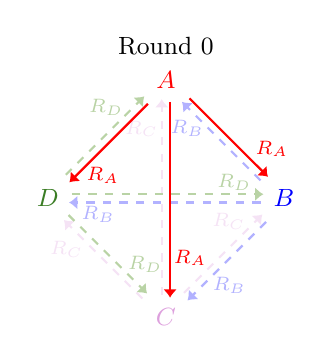
\begin{tikzpicture}[
		mycircle/.style= {
		fill,circle, inner sep=1pt
		},
		>={Latex[length=3pt,width=5pt]},<->,shorten <= 1pt,
		main node/.style={},
		font=\scriptsize,
		every path/.style={
	      thick
	  }
	]
		

	\newcommand*{\MainNum}{4}
	\newcommand*{\MainRadius}{1.5cm} 
	\newcommand*{\MainStartAngle}{180}
	
	% Print main nodes, node names: p1, p2, ...
	\coordinate (M) at (0,0);
	
	
	\node (u1) at ({-1*360/\MainNum + \MainStartAngle}:\MainRadius) {\small\ua{$A$}};
	\node[inner sep=1pt] (m_1) at ({-1*360/\MainNum + 135}:\MainRadius + 0.4cm) {};
	
	\node (u2) at ({-2*360/\MainNum + \MainStartAngle}:\MainRadius) {\small\ub{$B$}};
	\node[inner sep=1pt] (m_2) at ({-2*360/\MainNum + 135}:\MainRadius + 0.4cm) {};
	
	\node (u3) at ({-3*360/\MainNum + \MainStartAngle}:\MainRadius) {\small\uc{$C$}};
	\node[inner sep=1pt] (m_3) at ({-3*360/\MainNum + 135}:\MainRadius + 0.4cm) {};
	
	\node (u4) at ({-4*360/\MainNum + \MainStartAngle}:\MainRadius) {\small\ud{$D$}};
	\node[inner sep=1pt] (m_4) at ({-4*360/\MainNum + 135}:\MainRadius + 0.4cm) {};
	
	\node[above =1.7cm of M] {\small Round 0};


	

	

	

	\draw[->,dashed,blue!30,transform canvas={xshift=-1pt,yshift=-1pt}] (u2) -- node[below left,inner sep=-1pt, pos=0.75] {$R_B$} (u1); 
	\draw[->,dashed,blue!30,transform canvas={xshift=1pt,yshift=-1pt}] (u2) -- node[below right,inner sep=0pt,pos=0.7] {$R_B$} (u3); 
	\draw[->,dashed,blue!30,transform canvas={yshift=-1.5pt}] (u2) -- node[below,inner sep=1pt,pos=0.85] {$R_B$} (u4);
	
	\draw[->,dashed,Plum!30,transform canvas={xshift=-1.5pt}] (u3) -- node[left,inner sep=1pt,pos=0.85] {$R_C$} (u1); 
	\draw[->,dashed,Plum!30,transform canvas={xshift=-1pt,yshift=1pt}] (u3) -- node[above left,inner sep=0pt,pos=0.8] {$R_C$} (u2); 
	\draw[->,dashed,Plum!30,transform canvas={xshift=-1pt,yshift=-1pt}] (u3) -- node[below left,inner sep=0pt,pos=0.75] {$R_C$} (u4);
	
	\draw[->,dashed,OliveGreen!30,transform canvas={xshift=-1pt,yshift=1pt}] (u4) -- node[above left,inner sep=0pt, pos=0.75] {$R_D$} (u1); 
	\draw[->,dashed,OliveGreen!30,transform canvas={yshift=1.5pt}] (u4) -- node[above,inner sep=1pt,pos=0.85] {$R_D$} (u2); 
	\draw[->,dashed,OliveGreen!30,transform canvas={yshift=1.5pt}] (u4) -- node[above right,inner sep=0pt,pos=0.75] {$R_D$} (u3);		 	 

	\draw[->,red,transform canvas={xshift=1pt,yshift=1pt}] (u1) -- node[above right,pos=0.8,inner sep=1pt] {\ua{$R_A$}} (u2); 
	\draw[->,red,transform canvas={xshift=1.5pt}] (u1) -- node[right,inner sep=1pt,pos=0.8] {\ua{$R_A$}} (u3); 
	\draw[->,red,transform canvas={xshift=1pt,yshift=-1pt}] (u1) -- node[below right,pos=0.8,inner sep=0pt] {\ua{$R_A$}} (u4); 



\end{tikzpicture}


}

\end{standaloneframe}


\end{document}